\documentclass{article}
\usepackage[utf8]{inputenc}
\usepackage[margin=0.7in]{geometry}
\usepackage[colorlinks=true,
            linkcolor=red,
            urlcolor=blue,
            citecolor=red]{hyperref}
\usepackage{booktabs}
\usepackage{color}
\usepackage{graphicx}
\usepackage{float}
\usepackage{multirow}
\usepackage{amsmath}
\usepackage{graphicx}
\graphicspath{ {./figures/} }
\newcommand{\yueran}[1]{{\color{red}[Yueran: #1]}}
\newcommand{\zongyuan}[1]{{\color{blue}[Zongyuan: #1]}}

\title{\vspace{-1.5cm}5741 Project Final Report: H-1B Petition Analysis}
\author{Yueran Yang (yy595), Zongyuan Yuan (zy225)}
\date{}

\begin{document}
\maketitle
\vspace{-3em}

\section{Project Introduction}

\subsection{What is H1-B?}

The H-1B is a visa in the United States that allows U.S. employers to temporarily employ foreign workers in specialty occupations. Labor Condition Application (LCA) for the employee that includes information such as wages and job titles should be filed by the employer to the U.S. Department of Labor Employment and Training Administration to show that the employer wants to hire a foreign worker in a specific position for no more than 3 years. Once LCA is approved, the next stage of the H-1B is a random selection process often referred to as ”H-1B Lottery”. The lottery process will ultimately decide whether an applicant will get the H-1B visa. Effective 2022, a new policy will be applied to the lottery process, but the LCA stage remains unchanged. Due to the random nature of the lottery process, our project focuses only on the LCA stage.

\subsection{Project Goal}
The data set we are investigating in this project is the H1-B Visa Application data from \href{https://www.kaggle.com/abishekanbarasan1995/h1b-case-status-prediction}{Kaggle}. Using the historical data, our goal is to predict the status of an application given the background information of an applicant. Our goal is not only to come up with a model that can predict the outcome of a Labor Condition Application with high accuracy, but also to identify important factors that play the biggest roles in the application. In other words, we want to make our model not as a black box but interpretable.

\subsection{Project Significance}

Hiring a foreign worker for a position brings additional cost to an employer because the employer must pay for H-1B application fees and legal service fees. If an employer can know beforehand how likely their LCA for an employee is going to be approved, the employer can better decide whether they should hire a foreign candidate for a position. Our solution can not only make employers more informed about their risks in hiring a foreign but also save their cost by preventing filing an LCA that is unlikely going to be approved in the first place. This can save money and time for the companies to select their target employees for different positions. On the other hand, from the perspective of a job seeker, our solution can help him/her 1) compare between different job offers he/she has in terms of the chance of getting an H-1B 2) choose a job with more stable prospect 3) better plan their career path, which can make this two-way selection more efficient.

\section{Data Analysis}

\subsection{About the Dataset}
Our raw data, the H1b\_EDA\_data.csv file, has 2,448,729 rows and 36 columns with mixed data types containing numerical values, dates, categorical values, and texts. All features and counts of NA entry for each feature is shown in Table \ref{data_intro}. 

SOC\_CODE refers to Standard Occupation Classification, which is to classify workers into  categories.\footnote{See \url{https://www.bls.gov/soc/}} In this project, we use 2010 SOC System\footnote{See \url{https://www.bls.gov/soc/2010/2010\_major\_groups.htm}}. NAIC refers to North American Industry Classification. NAIC\_CODE is used to classify the business of a company \footnote{See \url{https://www.census.gov/naics/}}. 

CASE\_STATUS is the label in our project. It contains four statuses, CERTIFIED, WITHDRAWN, DENIED and CERTIFIED-WITHDRAWN. Thus, the goal of the project is to solve a multi-class classification problem.

\subsection{Preliminary Data Processing}

After conducting a preliminary investigation into each feature, we decided to discard the following features from our model:

% Please add the following required packages to your document preamble:
% \usepackage{graphicx}
\begin{table}[H]
\centering
\resizebox{\textwidth}{!}{%
\begin{tabular}{||c|c||cc}
\hline
\textbf{feature}       & \textbf{reason}        & \multicolumn{1}{c|}{\textbf{feature}}       & \multicolumn{1}{c||}{\textbf{reason}}        \\ \hline
Sector\_data           & Irrelevant information & \multicolumn{1}{c|}{WORKSITE\_POSTAL\_CODE} & \multicolumn{1}{c||}{Duplicate information}  \\ \hline
EMP\_STATE\_full       & Duplicate information  & \multicolumn{1}{c|}{YEAR}                   & \multicolumn{1}{c||}{Duplicate information}  \\ \hline
EMP\_STATE\_and\_city  & Simplicity             & \multicolumn{1}{c|}{WORKSITE\_COUNTY}       & \multicolumn{1}{c||}{Duplicate information}  \\ \hline
EMPLOYER\_PHONE        & Irrelevant information & \multicolumn{1}{c|}{WORKSITE\_CITY}         & \multicolumn{1}{c||}{Duplicate information}  \\ \hline
AGENT\_ATTORNEY\_NAME  & Irrelevant information & \multicolumn{1}{c|}{WAGE\_RATE\_OF\_PAY}    & \multicolumn{1}{c||}{Duplicate information}  \\ \hline
AGENT\_ATTORNEY\_CITY  & Irrelevant information & \multicolumn{1}{c|}{SOC\_NAME}              & \multicolumn{1}{c||}{Duplicate information}  \\ \hline
AGENT\_ATTORNEY\_STATE & Irrelevant information & \multicolumn{1}{c|}{EMPLOYER\_CITY}         & \multicolumn{1}{c||}{Duplicate information}  \\ \hline
JOB\_TITLE             & Duplicate information  & \multicolumn{1}{c|}{CASE\_NUMBER}           & \multicolumn{1}{c||}{Irrelevant information} \\ \hline
EMPLOYER\_POSTAL\_CODE & Duplicate information  &                                             &                                             \\ \cline{1-2}
\end{tabular}%
}
\end{table}

These features are discarded because either they are 1. irrelevant, 2. contain essentially the same information as other features, or 3. for the sake of simplicity of our model. Specifically, EMPLOYER\_PHONE apparently has nothing to do with the outcome of the application; SOC\_CODE already contains the information SOC\_NAME, JOB\_TITLE can provide, and EMP\_STATE\_abb already encodes the location information of the employer, so there is no need to include EMP\_STATE\_full and EMPLOYER\_POSTAL\_CODE. For EMP\_STATE\_and\_city, it contains too detailed information of the location of the employer. If we one-hot encode the feature, the dimension of the transformed dataset would be too large to handle. Also, there might be risk of over-fitting the data. Therefore, we are only interested in the state location of employers.

In the next step, we removed NA values for each remaining feature. From Table \ref{data_intro}, we can see that remaining features do not have a lot of missing values compared to the size of the dataset. Thus, removing NA values has minimal impact. 
\begin{table}[h] \label{tab: remaining-features}
\centering
\caption{Counts of NA for remaining feature}
\label{data_intro}
\begin{tabular}{|c|c|cc}
\hline
\textbf{Name}           & \textbf{NACount} & \multicolumn{1}{c|}{\textbf{Name}}        & \multicolumn{1}{c|}{\textbf{NACount}} \\ \hline
CASE\_STATUS            & 0                & \multicolumn{1}{c|}{total\_wage}          & \multicolumn{1}{c|}{0}                \\ \hline
CASE\_SUBMITTED         & 1                & \multicolumn{1}{c|}{NAIC\_CODE}           & \multicolumn{1}{c|}{2}                \\ \hline
DECISION\_DATE          & 0                & \multicolumn{1}{c|}{EMP\_STATE\_abb}      & \multicolumn{1}{c|}{0}                \\ \hline
EMPLOYMENT\_START\_DATE & 38               & \multicolumn{1}{c|}{SOC\_CODE}            & \multicolumn{1}{c|}{18}               \\ \hline
EMPLOYMENT\_END\_DATE   & 47               & \multicolumn{1}{c|}{EMPLOYER\_NAME}       & \multicolumn{1}{c|}{67}               \\ \hline
EMPLOYER\_COUNTRY       & 0                & \multicolumn{1}{c|}{VISA\_CLASS}          & \multicolumn{1}{c|}{0}                \\ \hline
PREVAILING\_WAGE        & 0                & \multicolumn{1}{c|}{FULL\_TIME\_POSITION} & \multicolumn{1}{c|}{7}                \\ \hline
PW\_UNIT\_OF\_PAY       & 0                & \multicolumn{1}{c|}{Worksite\_STATE\_abb} & \multicolumn{1}{c|}{16}               \\ \hline
WAGE\_UNIT\_OF\_PAY     & 19               &                                           &                                       \\ \cline{1-2}
\end{tabular}%
\end{table}

\subsection{Exploratory Data Analysis and Further Data Processing}

We first look at the distribution of CASE\_STATUS. From Figure \ref{fig:labels_distribution}, we can see that most of the applications are certified. Therefore, the labels of our data set is very unbalanced. Hence, when we are tuning our models, we must make sure that we are setting our parameters to handle the imbalance. 

Then we observed in Figure \ref{fig:prevailing_wage} that most applications are submitted by a small proportion of all companies. This means that the total demand for foreign workers concentrate in a small set of companies. If we simply apply one-hot encoding to the EMPLOYER\_NAME, we will again have an extremely high-dimensional transformed dataset. Therefore, based on the observation we made in Figure \ref{fig:prevailing_wage}, one approach to consider is to keep top 67 companies that submitted most applications which constitute around 80\% of total applications and group the rest of companies as others. But in this way, we might overlook the diversified needs for foreign workers of companies with smaller demand. Instead, we counted the number of applications submitted by each company so that it can reflect the difference in need for foreign workers while keeping all companies in our dataset. Using the count, we further calculate the priori rate for the 4 classes. 


\begin{figure}[h]
\centering
    \begin{minipage}{.32\textwidth}
        \centering
        \caption{Distribution of Labels}
        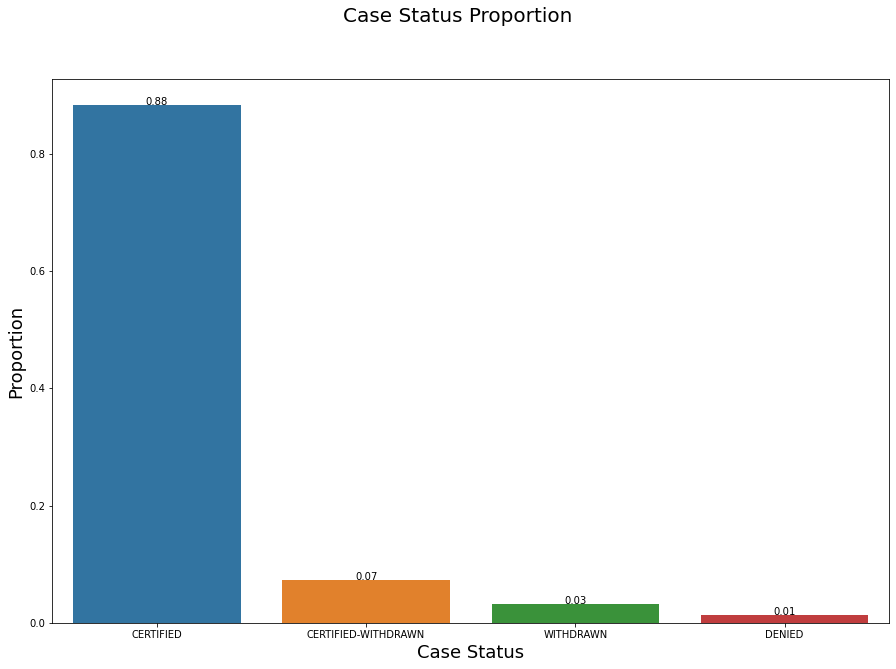
\includegraphics[width = \textwidth]{figures/fig11.png}
        \label{fig:labels_distribution}
    \end{minipage}
    \begin{minipage}{.32\textwidth}
        \centering
        \caption{Cumulative Proportion of Applications by Top Companies}
        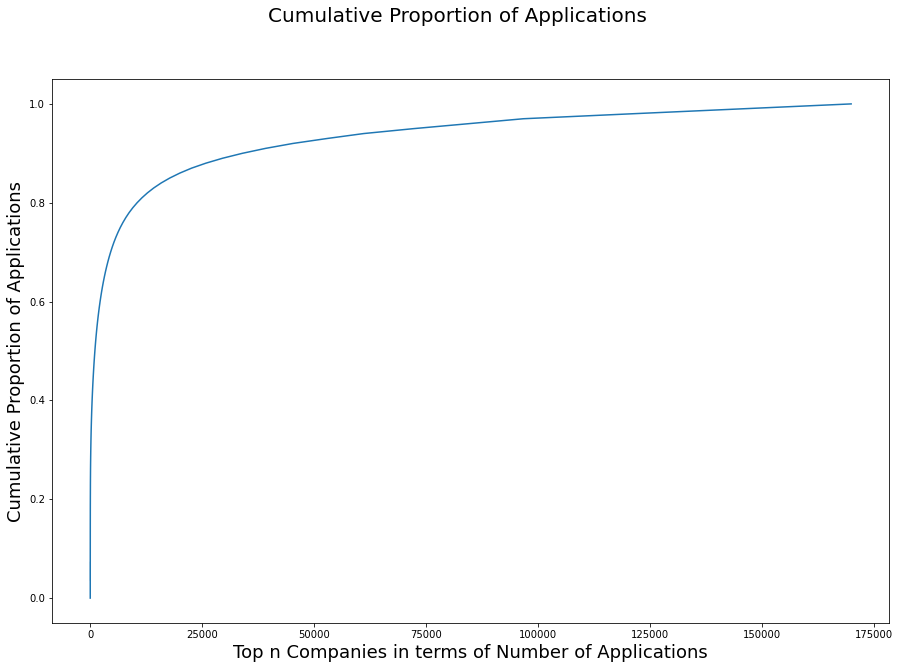
\includegraphics[width = \textwidth]{figures/fig1.png}
        \label{fig:prevailing_wage}
    \end{minipage}
    \begin{minipage}{.33\textwidth}
        \centering
        \caption{Wage Impact on Case Status}
        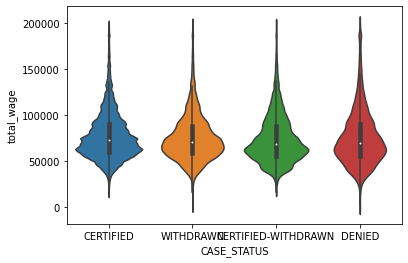
\includegraphics[width = \textwidth]{figures/wage_violin.png}
        \label{fig:violin}
    \end{minipage}
\end{figure}

Wage is an important indicator of the value of the job. The violin plot in Figure \ref{fig:violin} shows that average wages in certified applications are slightly higher than average wages in applications with other status. From the wage distribution plot below (Figure \ref{fig:wage_distribution}), we can see that most applications have wages from \$50,000 to \$100,000.

\begin{figure}[h]
\centering
    \begin{minipage}{.33\textwidth}
        \centering
        \caption{Wage Distribution}
        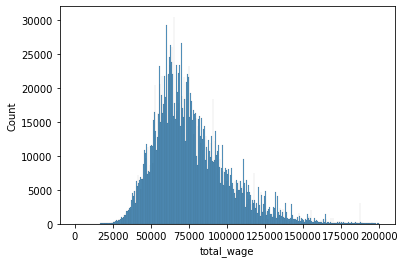
\includegraphics[width = \textwidth]{figures/wage_hist.png}
        \label{fig:wage_distribution}
    \end{minipage}
    \begin{minipage}{.34\textwidth}
        \centering
        \caption{Certified Rate by States}
        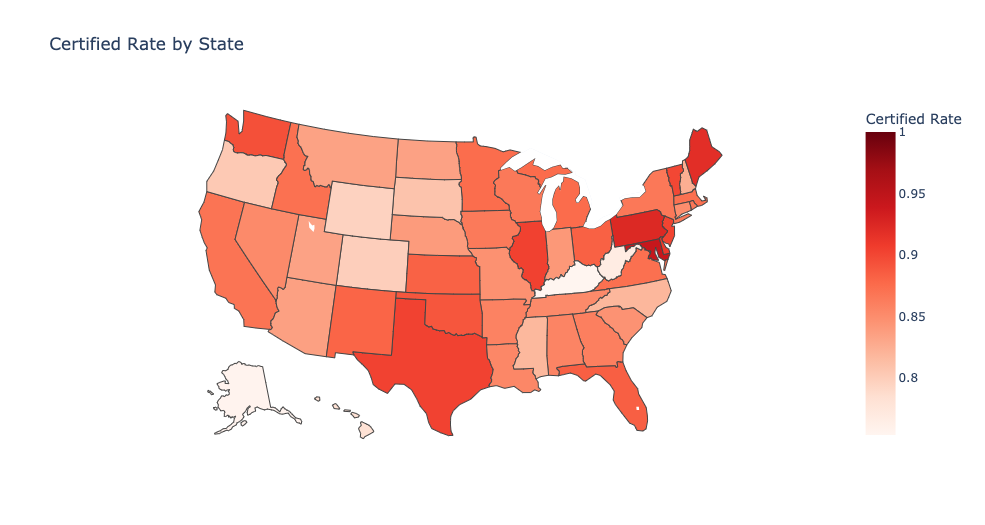
\includegraphics[width = \textwidth]{figures/fig3.png}
        \label{fig:state_distribution}
    \end{minipage}
    \begin{minipage}{.31\textwidth}
        \centering
        \caption{Industry Distribution}
        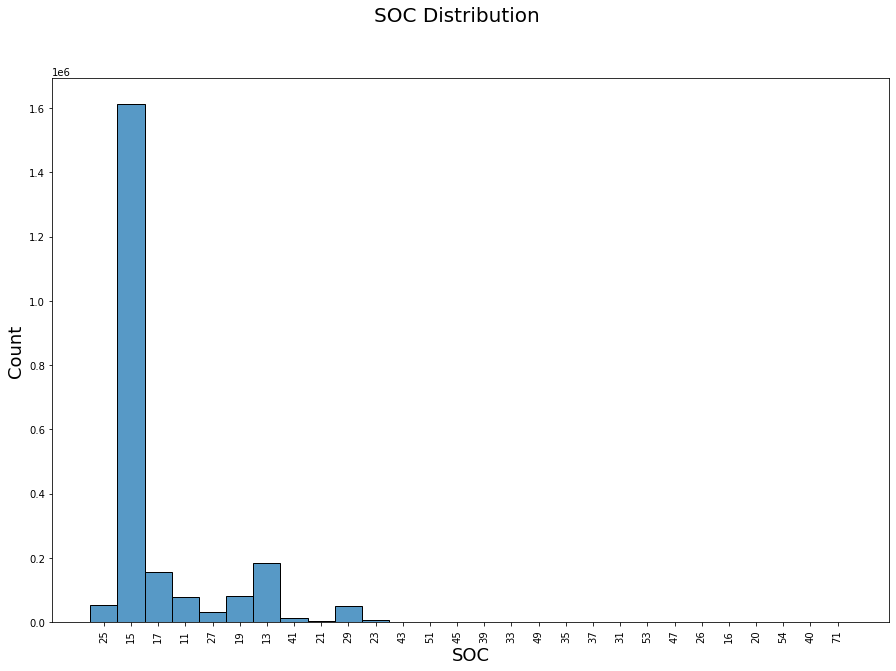
\includegraphics[width = \textwidth]{figures/fig8.png}
        \label{fig:industry_distribution}
    \end{minipage}
\end{figure}

Another important  factor  is  the  location  of  the employer. From Figure \ref{fig:state_distribution}, we can see that the applications from employers in some states are more likely to be certified than others. Additionally, as shown in Figure \ref{fig:industry_distribution}, the majority of the applications have SOC code that starts with 15 meaning that most of the applications are computer or software related.

Finally, we have transformed date-related features in Table 1 into duration. Then we normalized all numerical features. We randomly chose 70\% of the transformed dataset as our training set and used the rest as our test set.

\section{Methods}
In this section, we will discuss the models and sampling methods we have attempted as well as the metric we have chosen to evaluate the performance of our models.
\subsection{Models}
\subsubsection{Decision Tree}


This is a preliminary model we are using in the beginning, thus training data for this model is not down-sampled. Because of the large size of our training, we are only setting the depth of the tree to 2. This is because setting it larger than 2 would make the run-time of the algorithm unreasonably long. 

\subsubsection{Logistic Regression \& Linear SVM}
Logistic regression can only be used on binary classification. In multi-class problems, it simply generates 4 Logistic formulas to calculate the possibility for each class to be positive and chooses the most positive class as the final prediction. We tried Logistic Regression with L1, L2 and elastic regularization. But no regularization outperforms. Thus, the best model shown in the following evaluation is without regularization. 

The linear SVM's main idea is to find a most robust boundary between the two classes. We use linear SVM on binary settings by setting the maximum iteration to be 100 and the regularization parameter to be 0.01 on binary settings. 

We use pyspark to train the two models.

\subsubsection{Linear Discriminant Analysis (LDA) \& Quadratic Discriminant Analysis (QDA)}
The main idea of LDA is to train distinct models using data with the same label and to calculate $P(Y = k| X = x)$ using Bayes Theorem. The output is $\arg\max_{k \in K} P(Y = k| X = x)$. The prediction formula is 
$$
f_k(x) = \frac{1}{(2\pi)^{p/2} |\Sigma|^{0.5}} \exp \left\{-\frac{1}{2}(x-\mu_k)^T\Sigma^{-1}(x - \mu_k)\right\}
$$
where $\Sigma$ is the correlation matrix for the features, $\mu_k$ is the mean and p is the dimension of the features. QDA, different from LDA, uses $\Sigma_k$ instead of $\Sigma$ for all the classes. 

The two methods are expected to have more balanced performance on each label, but they do not work well in our problem. 

\subsubsection{Neural Network}
Neural Network use interaction between neurons in different layers to simulate the human thinking process. The parameters between each layers can be a huge matrix to quantify the interaction. The Neural Network used for both kinds of classification contain an input layer, two hidden layers with 256 and 64 neurons respectively, a dropout layer with drop rate 0.5 to avoid over-fitting and an output layer. The activation for the two hidden layers is ReLU. The output activation is sigmoid. In a dropout layer, some number of layer outputs are randomly ignored with probability as the drop rate. We used tensorflow platform to train this model. 
\begin{equation}
        \text{Sigmoid: }  {\displaystyle S(x)={\frac {1}{1+e^{-x}}}={\frac {e^{x}}{e^{x}+1}}=1-S(-x)} \quad
        \text{ReLU: }{\displaystyle f(x)=x^{+}=\max(0,x)}
\end{equation}

\subsubsection{AutoGluon\cite{agtabular}}
AutoGluon\cite{agtabular} is an AutoML library, which can efficiently try many traditional or modern machine learning methods on the data and tune the models automatically. The output of AutoGluon can be a leaderboard of different methods with test score, shown in Table \ref{tab:leaderboard}. 
\begin{table}[h]
\centering
\caption{Output of AutoGluon}
\label{tab:leaderboard}
\begin{tabular}{|c|c|c|c|}
\hline
\textbf{model}                & \textbf{score\_test} & \textbf{score\_val} & \textbf{pred\_time\_test} \\ \hline
\textbf{LightGBM\cite{NIPS2017_6449f44a}}             & 0.980459             & 0.98111             & 9.922074                  \\ \hline
\textbf{WeightedEnsemble\_L2} & 0.980254             & 0.981521            & 219.2322                  \\ \hline
\textbf{CatBoost\cite{prokhorenkova2019catboost}}             & 0.979415             & 0.980113            & 1.61188                   \\ \hline
\textbf{XGBoost \cite{10.1145/2939672.2939785}}              & 0.97929              & 0.979878            & 11.71829                  \\ \hline
\textbf{LightGBMXT}           & 0.978001             & 0.978235            & 69.85277                  \\ \hline
\textbf{NeuralNetFastAI}      & 0.974666             & 0.974539            & 71.79455                  \\ \hline
\textbf{KNeighborsDist}       & 0.96803              & 0.968262            & 27.45305                  \\ \hline
\textbf{KNeighborsUnif}       & 0.967789             & 0.967441            & 26.48503                  \\ \hline
\textbf{LightGBMLarge}        & 0.881571             & 0.881556            & 5.466261                  \\ \hline
\end{tabular}%

\end{table}

We use AutoGluon work as a very preliminary algorithm to help us to choose a model that can learn the mapping from features to labels. Thus, the training data for AutoGluon in the first step is non-down-sampled data which is the original training data, and the score is accuracy. 

We can see from Table \ref{tab:leaderboard} that the AutoML chose lightGBM is the best algorithm on the data. Furthermore, the other models picked out by AutoGluon are mostly tree-based ensemble models. We can conclude that tree-models are more suitable on this problem and the mapping from features to labels are very complicated. 

\textbf{Remark:} If we use balanced accuracy as score to evaluate each models, it turns out that the lightGBM is still the best model. The results is shown in figures/autogluon\_balanced.png . 

\subsubsection{Light Gradient Boosting Machine (LightGBM) \cite{NIPS2017_6449f44a}}
Now we look into the details of the best model picked by AutoGluon. LightGBM is a kind of gradient boosting decision tree algorithms, which improves the time efficiency and scalability on a large data set, compared to other gradient boosting decision trees. It was originally built by Microsoft. Gradient boosting decision tree is an ensemble of decision trees (weak predictors). It use a loss function to measure the residual between output and the true labels. The algorithm use the formula ($F_m$ is the current model and the $h_m$ is the current tree)
$$
F_m(x) = F_{m-1}(x) + \gamma_mh_m(x) 
$$
to generate a ensemble model. And the $\gamma_m$ is calculated by minimize the loss function, which is 
$$
\gamma_m = \arg\min \sum_{i = 1}^n L(y_i, F_{m-1}(x_i) + \gamma h_m(x_i))
$$

We used lightGBM package in python to train the model. In LightGBM, when it is dealing with binary classification problem, the model can handle imbalanced data by setting is\_unbalanced to be True. This will add weights on the positive label to balance the classes, assuring that the model will not favor one specific class. Thus, we are trying two different objectives in LightGBM, one is to the original labels, which is a multi-class problem and the other is to use the one-vs-all (ova) method to deal with this multi-class classification. When using multi-class objective, we use our down-sampled data as training data. When using the ova method, we set the inner parameter is\_unbalanced to be True. 

\subsection{Down-Sampling} \label{down-sampling}
The method is used to improve the performance of previous methods on each class. The original data is very imbalanced. About 90\% of the labels are certified, and only approximately 1\% of the labels are denied. In order to make our model more generalized to all the classes. We manually adjust the training data to make sure it contains the sample number of samples for each class. 

There are totally 24,748 denied samples in our training data. Thus, we randomly sample 24,748 samples from the other 3 classes respectively, which makes the down-sampled training data to have 98,992 samples. The down-sampled training data will not be used in LDA and QDA because the prior possibility works as an essential part in both models. Also, the down-sampled method is not used on Decision Tree and LightGBM with the one-vs-all objective, as we mentioned before. The results of decision trees can be used to compare the binary classification and the 4-class classification. 

For binary classification, we use the same method, but in this case, we only have two classes. The down-sampled data is used when there is a huge gap between accuracy on 1 and on 0. Thus, the down-sampled data is used on SVM, Neural Network and Logistic Regression. 

\subsection{Metrics} \label{metrics}
Since the data is very imbalanced, especially on denied status, instead of using pure accuracy to measure our models, we are using average accuracy (balanced accuracy) to make sure the final model we get will not favor any class. The balanced accuracy is the average of accuracy on each class. The balanced accuracy is only used in the last evaluation of each model, not in the training process as we already use down-sampled training data or other balanced methods to train the models. The average accuracy is defined as follows:
\begin{equation} \label{eq:1}
        \frac{1}{4}\left(\text{accuracy}_\text{certified} + \text{accuracy}_\text{certified-withdrawn} + \text{accuracy}_\text{withdrawn} + \text{accuracy}_\text{denied}\right)
\end{equation}
\section{Fairness Analysis}

Our features do not contain demographic information such as age, race and gender. Therefore, our models would not favor applicants from any demographic group. However, since our dataset is very imbalanced, if we do not add extra touch to our models, our predictions might favor certified cases more. Thus, we have taken the following two measures to ensure the fairness of our models.

1. Down sampling: Data with each label constitutes an equal proportion in our training set

2. Average accuracy: We care about the accuracy of the model for applications with different case status equally. 

\section{Results}
\subsection{Model Evaluation}
\subsubsection{Binary Classification}
We can transform the certified status into 1 and the other three labels into 0 to make the original problem into a binary classification. The ratio of 1 and 0 would be 88:12, which is not as imbalanced as the original 4 classes. The results of each model are shown in Table \ref{tab: eva2}

If we turn the models into binary classification, we can see that the accuracy of decision is high enough to separate the two classes. And the accuracy on the failed and the certified class is 0.91784763 and 0.98987939 respectively, which means that the decision tree can learn the data well. 
\begin{table}[H]
\centering
\caption{Evaluations of each model for binary classification}
\label{tab: eva2}
\begin{tabular}{|c|c|c|}
\hline
\multirow{2}{*}{\textbf{Models}} & \multirow{2}{*}{\textbf{Training Accuracy}} & \multirow{2}{*}{\textbf{Test Accuracy}} \\
                                 &                                                       &                                                 \\ \hline
\textbf{Decision Tree}           & 0.9820                                                & 0.9820                                          \\ \hline
\textbf{SVM}                     & 0.7885                                                & 0.8417                                          \\ \hline
\textbf{Neural Network}          & 0.8933                                                & 0.9818                                          \\ \hline
\textbf{Logistic Regression}     & 0.7908                                                & 0.8539                                          \\ \hline
\textbf{QDA}                     & 0.8275                                                & 0.8268                                          \\ \hline
\textbf{LDA}                     & 0.9303                                                & 0.9305                                          \\ \hline
\end{tabular}%
\end{table}
These are not the major results in our projects, so we are not going to dig into these results. 

\subsubsection{4-class classification}
The performance of the models are shown in Table \ref{tab: eva4}. According to the performance of each model and the output of the preliminary AutoGluon algorithm, the mapping from features to labels are so complicated that more flexible models (with more complexity) work better on this problem. Also, the tree-based models generally work better than other kinds of model. Linear models are too simple to learn the data. 
\begin{table}[H]
\centering
\caption{Evaluations of each model for 4-class classification}
\label{tab: eva4}
\resizebox{\textwidth}{!}{%
\begin{tabular}{|c|c|c|cccc|}
\hline
\multirow{2}{*}{\textbf{Models}}    & \multirow{2}{*}{\textbf{\begin{tabular}[c]{@{}c@{}}Training Average  \\ Accuracy\end{tabular}}} & \multirow{2}{*}{\textbf{\begin{tabular}[c]{@{}c@{}}Test Average \\ Accuracy\end{tabular}}} & \multicolumn{4}{c|}{\textbf{Test Accuracy}}                                                                                                             \\ \cline{4-7} 
                                    &                                                                                                 &                                                                                            & \multicolumn{1}{c|}{\textbf{Certified}} & \multicolumn{1}{c|}{\textbf{Certified-Withdrawn}} & \multicolumn{1}{c|}{\textbf{Denied}} & \textbf{Withdrawn} \\ \hline
\textbf{lightGBM (OVA)}             & 0.8919                                                                                          & 0.8804                                                                                     & \multicolumn{1}{c|}{0.9603}             & \multicolumn{1}{c|}{0.9650}                       & \multicolumn{1}{c|}{0.7749}          & 0.8215             \\ \hline
\textbf{lightGBM  (multiclass)}     & 0.8976                                                                                          & 0.8860                                                                                     & \multicolumn{1}{c|}{0.9170}             & \multicolumn{1}{c|}{0.9532}                       & \multicolumn{1}{c|}{0.8522}          & 0.8214             \\ \hline
\textbf{Logistic Regression (best)} & 0.6070                                                                                          & 0.6064                                                                                     & \multicolumn{1}{c|}{0.9708}             & \multicolumn{1}{c|}{0.8611}                       & \multicolumn{1}{c|}{0.4034}          & 0.1903             \\ \hline
\textbf{LDA (without downsampling)} & 0.5967                                                                                          & 0.5980                                                                                     & \multicolumn{1}{c|}{0.9559}             & \multicolumn{1}{c|}{0.6993}                       & \multicolumn{1}{c|}{0.4611}          & 0.2757             \\ \hline
\textbf{Decision Tree (not down-sampled)}              & 0.6659                                                                                          & 0.6674                                                                                     & \multicolumn{1}{c|}{0.9900}             & \multicolumn{1}{c|}{0.9343}                       & \multicolumn{1}{c|}{0.7452}          & 0.0000             \\ \hline
\textbf{Neural Network}              & 0.8760                                                                                          & 0.8352                                                                                     & \multicolumn{1}{c|}{0.8733}             & \multicolumn{1}{c|}{0.9559}                       & \multicolumn{1}{c|}{0.7689}          & 0.7428             \\ \hline
\end{tabular}%
}
\end{table}

The reason that we are not using binary classification to analyze the certified rate in the following content is that the huge performance gap of Decision Tree on both problem shows that the binary classification may ignore some relations among features and labels. In order to use a more precise and reasonable model on each feature, we use lightGBM(ova) in the following analysis, since it is using model labels to train compared to other down-sampled models and having relatively higher average accuracy.. 

\subsection{Analysis on lightGBM(ova)} 
From Figure \ref{fig:importance}, we can see that there is a huge gap between the importance of the top 9 features and the other features. Thus, we want to dig into the top 9 features. Also the Certified rate, certified-withdrawn rate, denied rate and withdrawn rate are highly related as their sum must be 1. In this case, we want to analyze certified chance. Thus, we will only specifically look into priori certified rate. 
\begin{figure}[H]
    \centering
    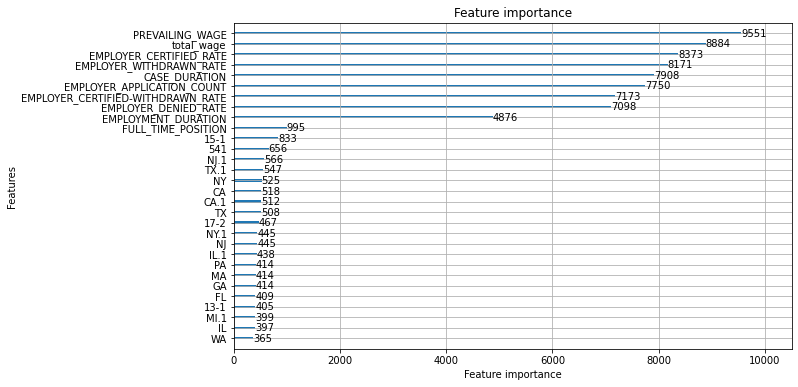
\includegraphics[width= .8\textwidth]{output_106.png}
    \caption{Top 30 important features}
    \label{fig:importance}
\end{figure}
\subsection{Feature Analysis}
By analyzing the impact of these features in our model, we used artificial data, generated by randomly sampling 10 data from the test data and changing the value of the feature that we want to analyze while keeping the other features fixed. Then, we see the trend of the predicted possibility to be certified. The lines in the following figures are different samples from the test data. 

\noindent\textbf{Total Wage \& Prevailing Wage}

From Figure \ref{fig:total_wage}, if your wage is around average or slightly above average, there will be a slight increase in certified probability. But when it is too large, the predicted certified probability will decrease. The reason for the phenomena might be that there is some correlation between wage and other features, so when we adjust the wage manually, it will cause inconsistency to other features, which can be unreasonable to the U.S. Department of Labor Employment. And there might be some special position that cannot be approved to hire a foreign worker with a very high wage in our data.  

Prevailing wages are showing the similar trend as the total wage. 

\noindent\textbf{Employer Certified Rate}

This is a priori possibility for an employee in a company to be certified. To analyze the impact, we adjust the priori possibility from 0.5 to 1. In the meantime, to make the other three priori possibility work, we manually set the denied rate to be 1 - the certified rate we set and the other two to be 0. We can see from Figure \ref{fig:employer} that the chance to be certified for an individual is highly related to the employer’s total priori certified rate. The higher the rate, more possible for an employee to be certified. 

\noindent\textbf{Case Duration}

From Figure \ref{fig:case_duration}, if you have an extreme case duration, the probability to be certified is very low. We can use the result to predict the final status, if you are waiting too long, you might be denied. If result comes out in a very short time, either you withdraw your application, or you might be denied. 

\noindent\textbf{Employer’s application count}

From Figure \ref{fig:count}, application counts have a slight impact on the final status. We can still conclude that more applications before, there will be a higher chance to be certified for an employee. 

\noindent\textbf{Employment Duration}

From Figure \ref{fig:employment_duration}, there is no obvious impact on the certified probability. We can see slight decrease when the employment duration is very large. It can be because that the application happens in the very beginning of the employment (always in the beginning of OPT with longer employment duration), which would cause high denied rate, since being denied or withdrawn means that the person cannot continue to work in US. 
\begin{figure}[H]
\centering
    \begin{minipage}{.30\textwidth}
        \centering
        \caption{Total Wage}
        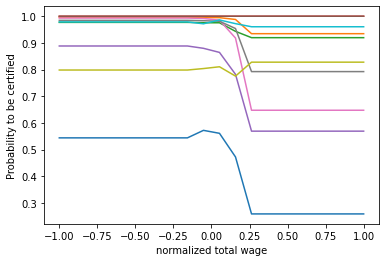
\includegraphics[width = \textwidth]{figures/total_wage.png}
        \label{fig:total_wage}
    \end{minipage}
    \begin{minipage}{.31\textwidth}
        \centering
        \caption{Prevailing Wage}
        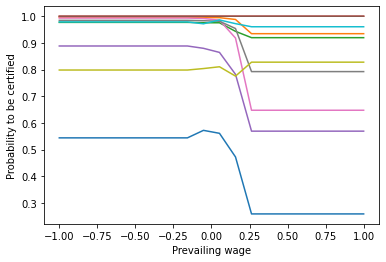
\includegraphics[width = \textwidth]{figures/prevailing_wage.png}
        \label{fig:prevailing_wage}
    \end{minipage}
    \begin{minipage}{.31\textwidth}
        \centering
        \caption{Employer certified rate}
        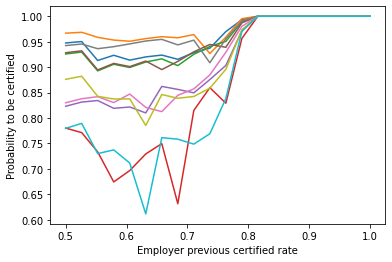
\includegraphics[width = \textwidth]{figures/Employer_certified_rate.png}
        \label{fig:employer}
    \end{minipage}
    
    \begin{minipage}{.30\textwidth}
        \centering
        \caption{Case Duration}
        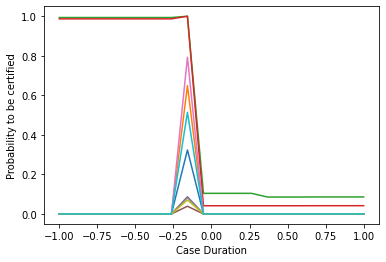
\includegraphics[width = \textwidth]{figures/case_duration.png}
        \label{fig:case_duration}
    \end{minipage}
    \begin{minipage}{.31\textwidth}
        \centering
        \caption{Employer's application count}
        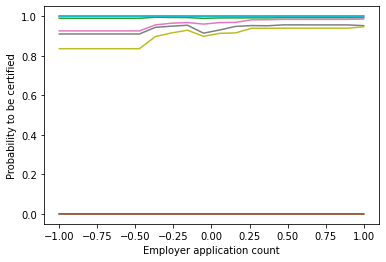
\includegraphics[width = \textwidth]{figures/application_count.png}
        \label{fig:count}
    \end{minipage}
    \begin{minipage}{.31\textwidth}
        \centering
        \caption{Employment Duration}
        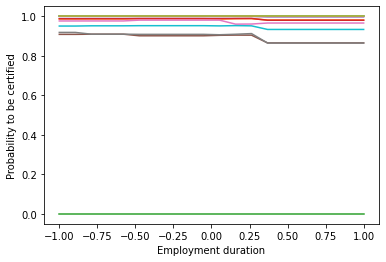
\includegraphics[width = \textwidth]{figures/employment_duration.png}
        \label{fig:employment_duration}
    \end{minipage}
\end{figure}
\section{Weapon of Math Destruction \cite{o2016weapons}}
A model is considered a Weapon of Math Destruction (WMD) if it satisfies one of the following three criterion: 1. the outcome of a model is not easily measurable 2. can have negative consequences 3. has self-fulfilling feedback loop. Our model is not a WMD because it a has measurable outcome which is the status of an application. Secondly, our model has no negative consequence because most of the applications are approved ,and our model focuses on helping those who might not be approved become aware of their risks. Furthermore, our model has no prominent self-fulfilling feedback loop. Whether an H1-B is going to be approved is determined entirely the competency of the employee and the industry demand. These two factors are unlikely to be affected by the prediction of the H1-B application status.  
\section{Conclusion}
In this project, we explored the Labor Condition Application data and attempted various models to predict the case status of LCA application. The performance of each model is summarized in Table \ref{tab: eva4}. The internal process of LCA application is very complicated. Based on our attempts, we found that tree-based models work better. More generally, linear models do not work well on our dataset while more complicated models have better performance. From a company's perspective, to increase the chance of being certified, it should offer a reasonable salary to its foreign employee but not too high. From the perspective of a foreign worker, to increase the chance of being certified, he/she should choose a big company that submitted more previous applications and/or choose a company with higher priori certified probability. But most importantly, one should increase his/her own competency to be accepted by a better company to increase his/her chance to be certified. 

\section{Future Work}
In the analysis aspect, first, we trained a model that can predict the four class equivalently. The model can be further used in analyze the other two labels, which is withdrawn and certified withdrawn to understand specific pattern that may indicate the withdrawing. Secondly, we used synthetic data to analyze the feature impacts in our model. The model can be further evaluated and interpreted by the real data. 

In the training aspect, more methods can be tried to deal with these imbalanced labels. Also, the correlation among features can be removed to make the model more accurate, but the detection of the correlation can be very difficult since most features are categorical in the original data. 

\bibliography{ref}
\bibliographystyle{plain}



\end{document}
